\chapter{Results}
This chapter presents results obtained during the research process. Here, outcome of each implemented technique is illustrated, with a detailed description of its generation method and initial analysis. Additionally, to present wider contexts, details of training process of each artificial neural network are discussed in this section.\\

To ensure comparability of results obtained from each implemented method, all details related to network topologies and training process, except for those that are specific for analyzed approach, should be unified. It is especially important in case of techniques which incorporate autoencoder idea, as dimensionality of latent space, may have great impact on final results, and therefore should be kept the same for each method. Such assumptions ensure that all differences in results arise from exceptional quality of particular technique.\\

Additionally, to be able to fairly evaluate effectiveness of each implemented method, for all cases, the same set of images was used to generate final results. Images come from the original dataset and were selected to cover different head positions, facial expressions and lightning conditions.

\newpage
\section{Autoencoder}
\label{Results_Autoencoder}
The encoder and decoder XY were trained as long, as there was a noticeable improvement in loss function, which in this particular case was 150 epochs, as shown in figure \ref{fig:ae_decoderXY}. If the training process would be prolonged, overfitting would occur and the encoder would lose the generalization ability. Decoder X and decoder Y were trained far longer, past the point where loss function has no noticeable improvement, which in this case was 500 epochs. During training process, trained models were saved every 50 epochs, and later, to generate final results, the most effective models were selected.

\begin{figure}[H]
\centering
\begin{subfigure}{.5\textwidth}
  \centering
  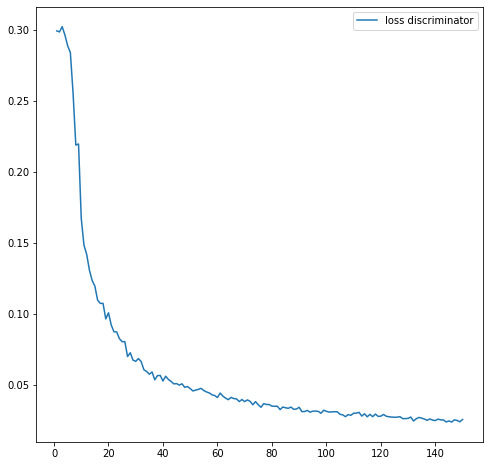
\includegraphics[width=1\linewidth]{ae_decoderXY_loss.png}
  \caption{Loss function}
  \label{subfig:ae_decoderXY_loss}
\end{subfigure}%
\begin{subfigure}{.5\textwidth}
  \centering
  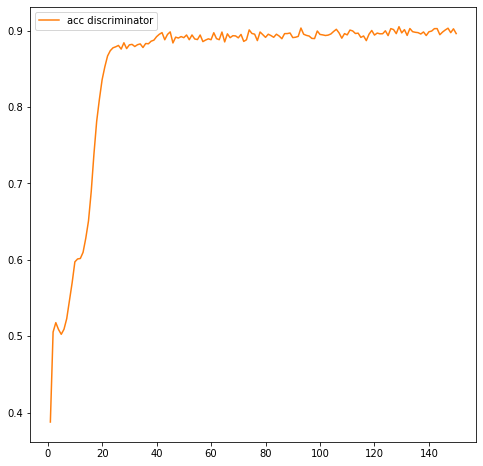
\includegraphics[width=1\linewidth]{ae_decoderXY_acc.png}
  \caption{Accuracy}
  \label{subfig:ae_decoderXY_acc}
\end{subfigure}
\caption{Training process of AE encoder and decoder XY}
\label{fig:ae_decoderXY}
\end{figure}

Below, results of trained models, generated for each person are presented. First column from the left contains original images to be encoded into latent vectors. Following columns present faces generated by respective decoders, from obtained feature maps. Actual deepfakes are presented in the last column, while remaining columns act as a frame of reference.\\

As might be observed in the figures below, autoencoders method generates deepfakes with certain similarity to the original images. Although the head position and overall resemblance are correctly depicted in majority of cases, fake images are slightly blurred and do not portray facial expressions accurately. Additionally, as for example in figure \ref{fig:ae_y_scene2_350}, in some cases, certain artifacts are present in the pictures.

\subsection{Subject X}

\begin{figure}[H]
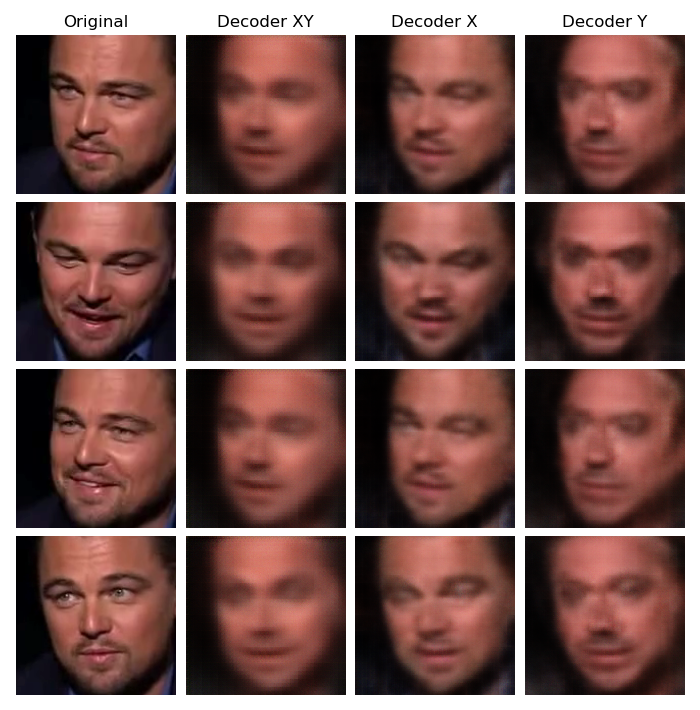
\includegraphics[width=10cm] {Results/ae_x_scene1_350.png}
\centering
\caption{Sample 1 from subject X after 350 epochs}
\label{fig:ae_x_scene1_350}
\end{figure}

\begin{figure}[H]
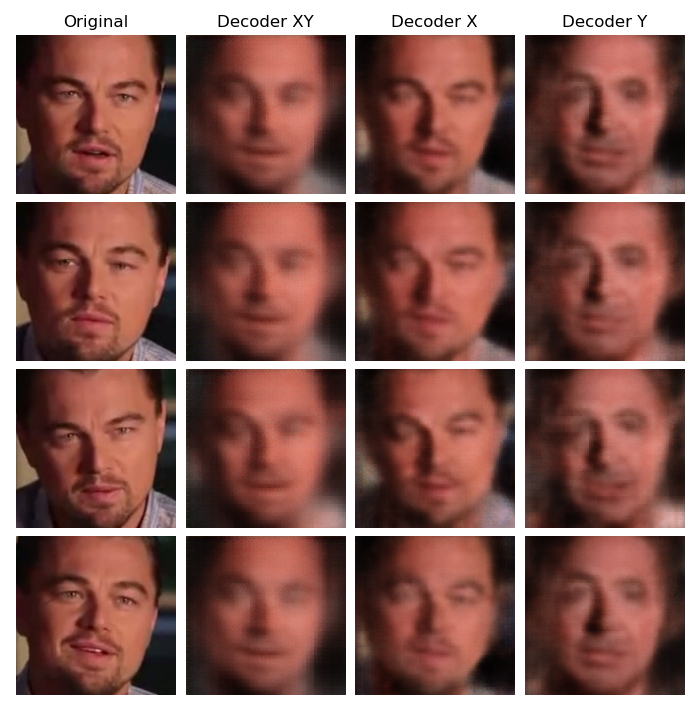
\includegraphics[width=10cm] {Results/ae_x_scene2_350.png}
\centering
\caption{Sample 2 from subject X after 350 epochs}
\label{fig:ae_x_scene2_350}
\end{figure}

\begin{figure}[H]
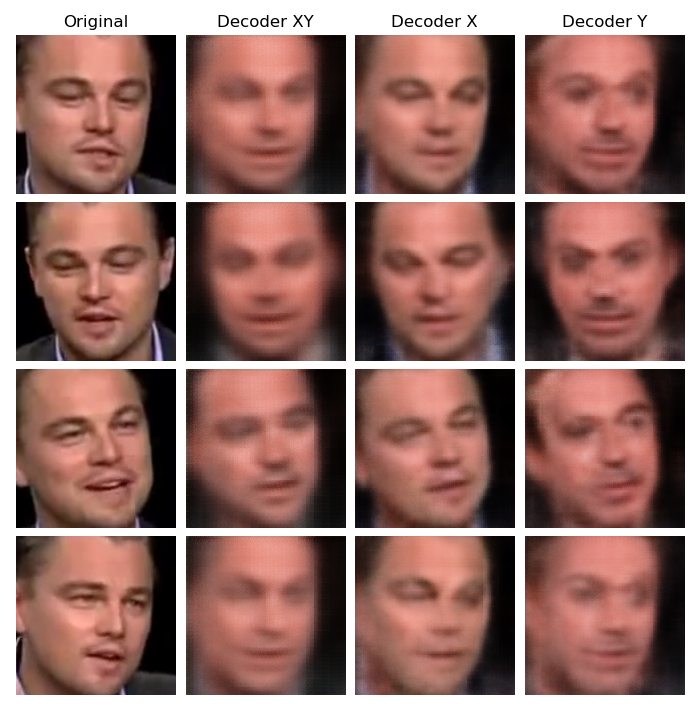
\includegraphics[width=10cm] {Results/ae_x_scene3_350.png}
\centering
\caption{Sample 3 from subject X after 350 epochs}
\label{fig:ae_x_scene3_350}
\end{figure}

\begin{figure}[H]
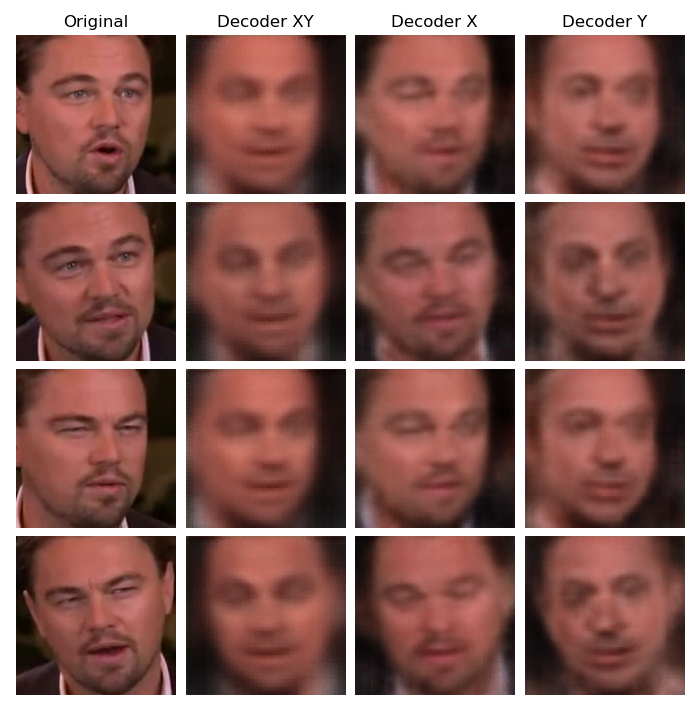
\includegraphics[width=10cm] {Results/ae_x_scene4_350.png}
\centering
\caption{Sample 4 from subject X after 350 epochs}
\label{fig:ae_x_scene4_350}
\end{figure}

\subsection{Subject Y}

\begin{figure}[H]
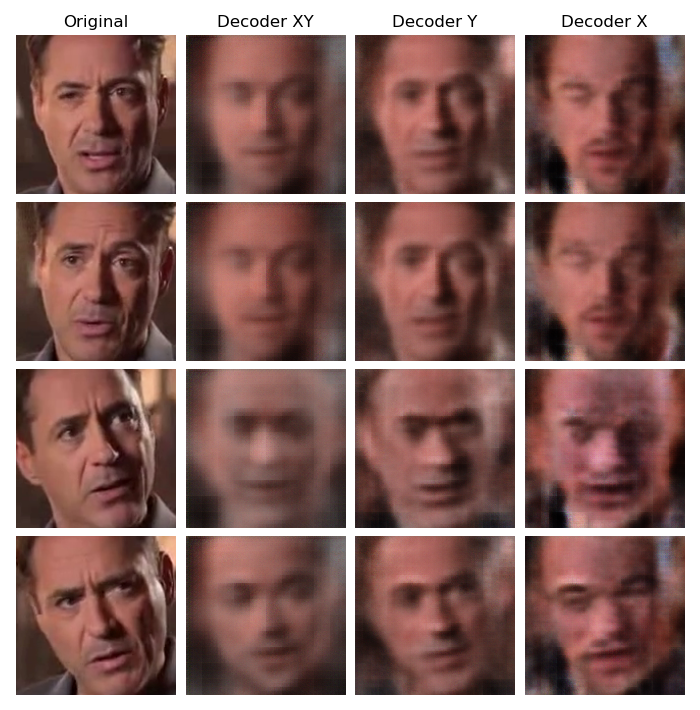
\includegraphics[width=10cm] {Results/ae_y_scene1_350.png}
\centering
\caption{Sample 1 from subject Y after 350 epochs}
\label{fig:ae_y_scene1_350}
\end{figure}

\begin{figure}[H]
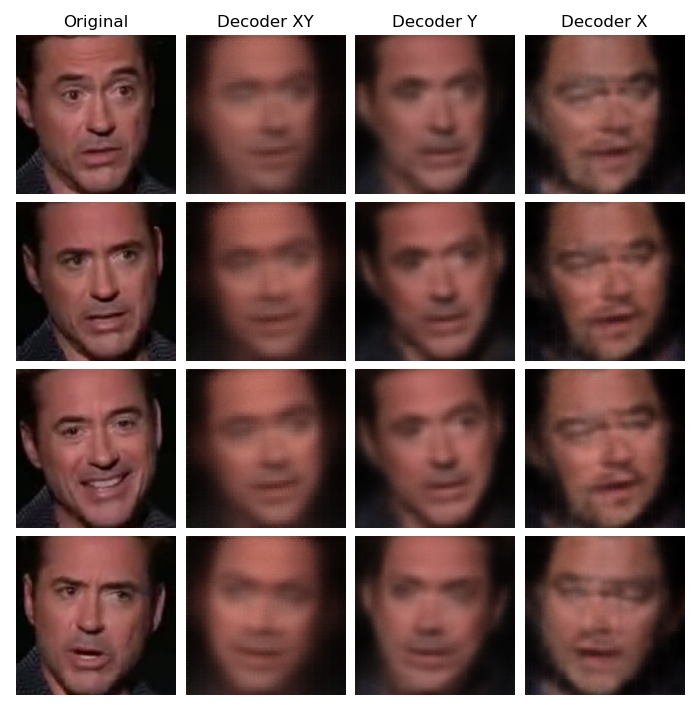
\includegraphics[width=10cm] {Results/ae_y_scene2_350.png}
\centering
\caption{Sample 2 from subject Y after 350 epochs}
\label{fig:ae_y_scene2_350}
\end{figure}

\begin{figure}[H]
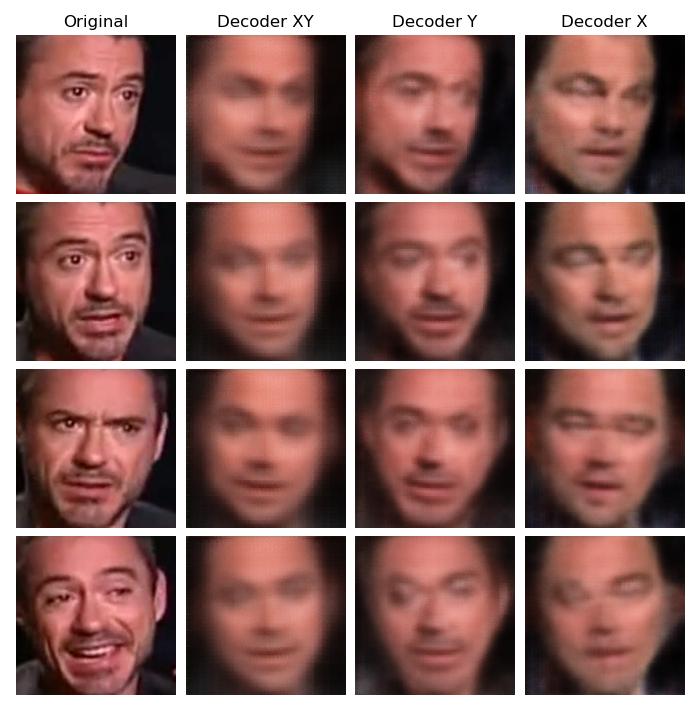
\includegraphics[width=10cm] {Results/ae_y_scene3_350.png}
\centering
\caption{Sample 3 from subject Y after 350 epochs}
\label{fig:ae_y_scene3_350}
\end{figure}

\begin{figure}[H]
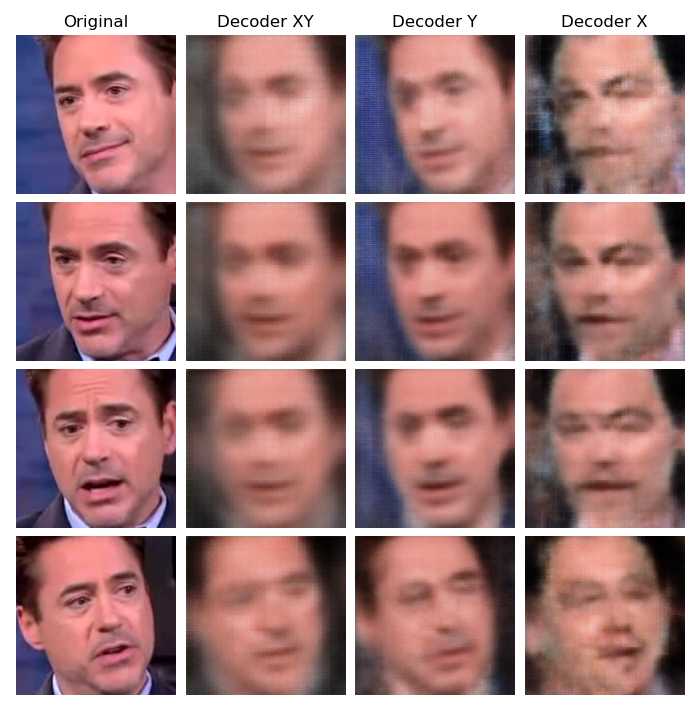
\includegraphics[width=10cm] {Results/ae_y_scene4_350.png}
\centering
\caption{Sample 4 from subject Y after 350 epochs}
\label{fig:ae_y_scene4_350}
\end{figure}

\section{Variational autoencoder}
\label{Results_Variational_Autoencoder}
Training process for variational autoencoders method were the same as the one described in senction \ref{Results_Autoencoder}. The encoder and decoder XY were trained were trained for 150 epochs, as shown in figure \ref{fig:vae_decoderXY}. Decoder X and decoder Y were trained for 800 epochs and during training process, trained models were saved every 50 epochs. Later, to generate final results, the most effective models were selected.

\begin{figure}[H]
\centering
\begin{subfigure}{.5\textwidth}
  \centering
  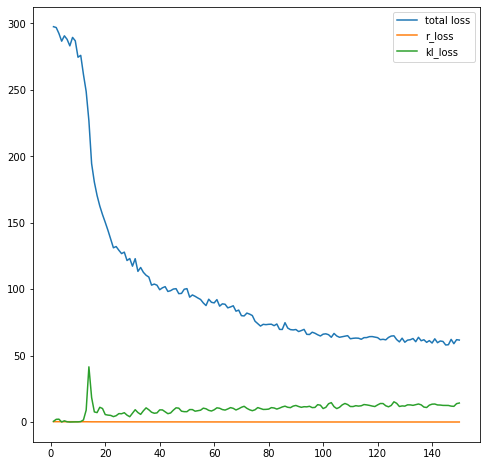
\includegraphics[width=1\linewidth]{vae_decoderXY_loss.png}
  \caption{Loss function}
  \label{subfig:vae_decoderXY_loss}
\end{subfigure}%
\begin{subfigure}{.5\textwidth}
  \centering
  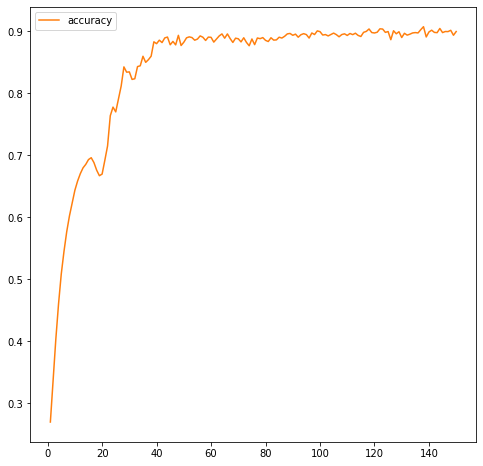
\includegraphics[width=1\linewidth]{vae_decoderXY_acc.png}
  \caption{Accuracy}
  \label{subfig:vae_decoderXY_acc}
\end{subfigure}
\caption{Training process of VAE encoder and decoder XY}
\label{fig:vae_decoderXY}
\end{figure}

Results presented below are in the same form as in previous section, generated over the same set of images. Deepfakes obtained from variational autoencoders method are of similar quality as those from section \ref{Results_Autoencoder}. One major difference, that arises from unique properties of VAE method, is the absence of artifacts in generated images. Except this improvement, blurriness and lack of correct facial expressions remain.

\subsection{Subject X}

\begin{figure}[H]
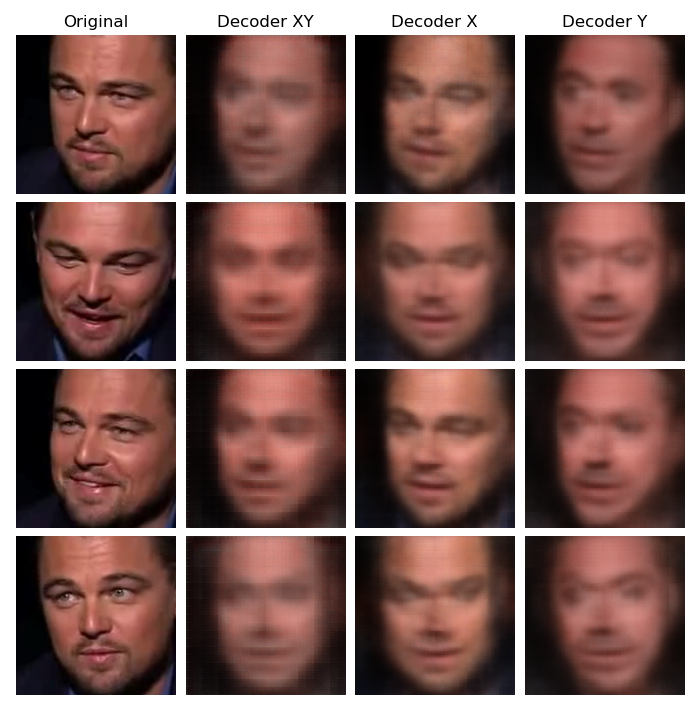
\includegraphics[width=10cm] {Results/vae_x_scene_1_800.png}
\centering
\caption{Sample 1 from subject X after 800 epochs}
\label{fig:vae_x_scene1_800}
\end{figure}

\begin{figure}[H]
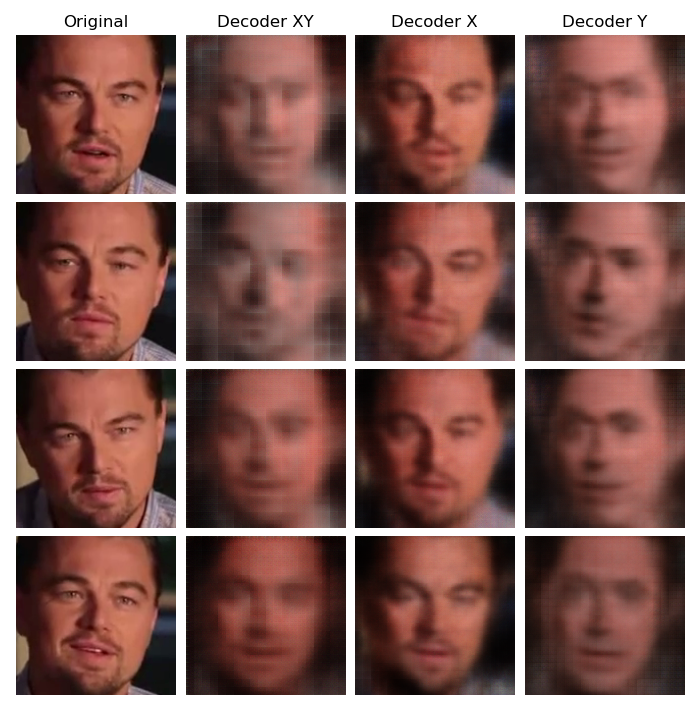
\includegraphics[width=10cm] {Results/vae_x_scene_2_800.png}
\centering
\caption{Sample 2 from subject X after 800 epochs}
\label{fig:vae_x_scene2_800}
\end{figure}

\begin{figure}[H]
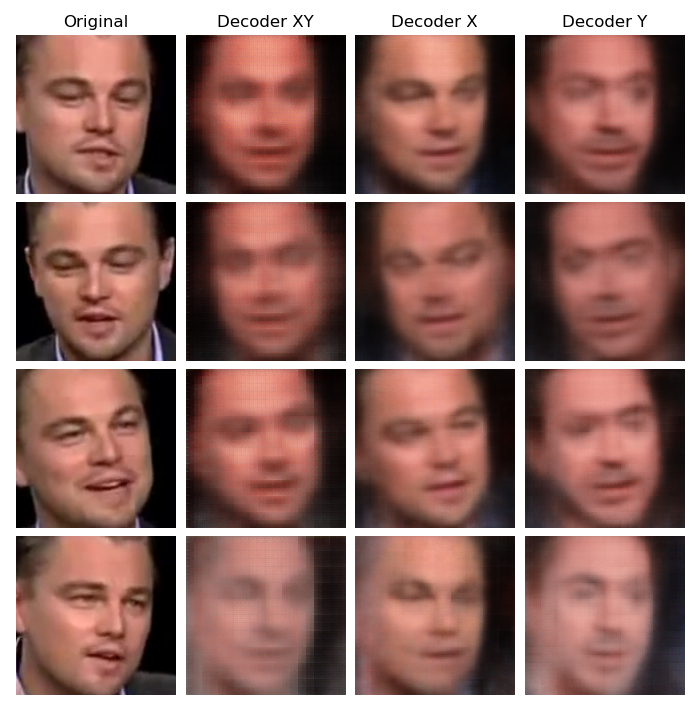
\includegraphics[width=10cm] {Results/vae_x_scene_3_800.png}
\centering
\caption{Sample 3 from subject X after 800 epochs}
\label{fig:vae_x_scene3_800}
\end{figure}

\begin{figure}[H]
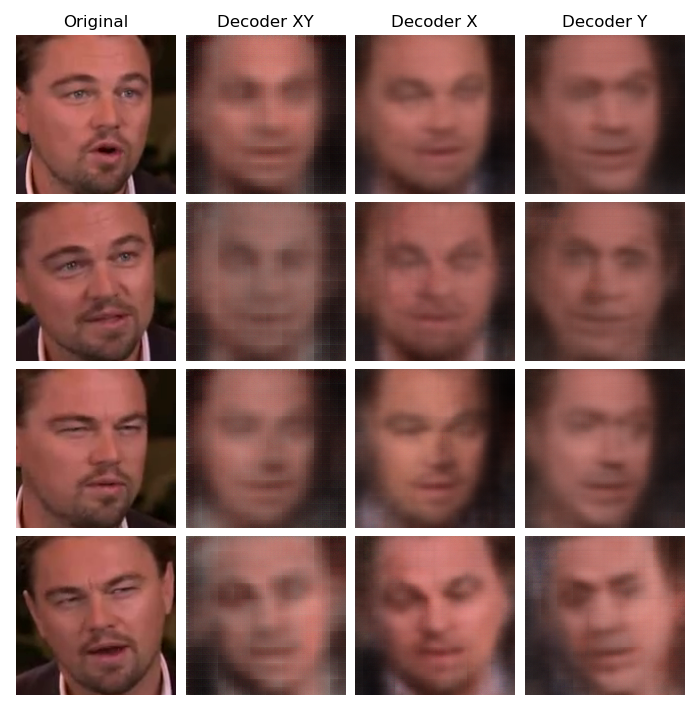
\includegraphics[width=10cm] {Results/vae_x_scene_4_800.png}
\centering
\caption{Sample 4 from subject X after 800 epochs}
\label{fig:vae_x_scene4_800}
\end{figure}

\subsection{Subject Y}

\begin{figure}[H]
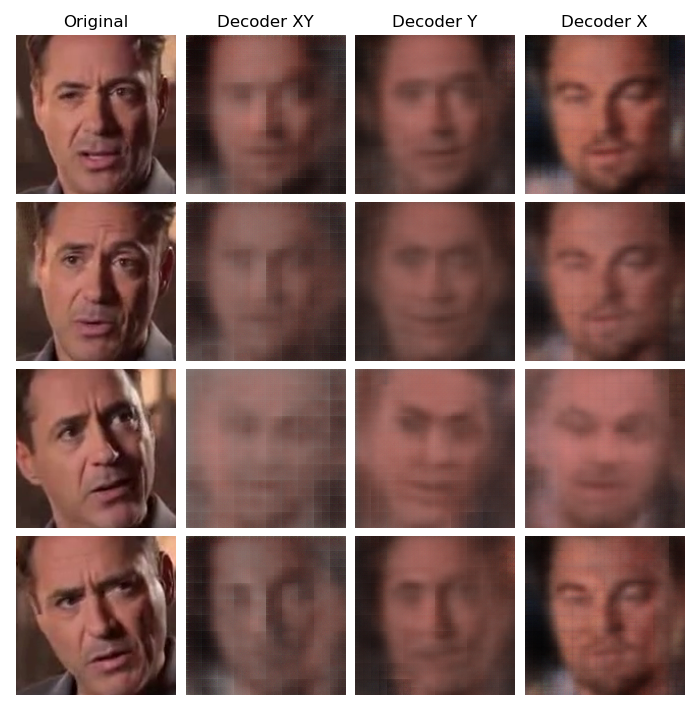
\includegraphics[width=10cm] {Results/vae_y_scene_1_600.png}
\centering
\caption{Sample 1 from subject Y after 600 epochs}
\label{fig:vae_y_scene1_600}
\end{figure}

\begin{figure}[H]
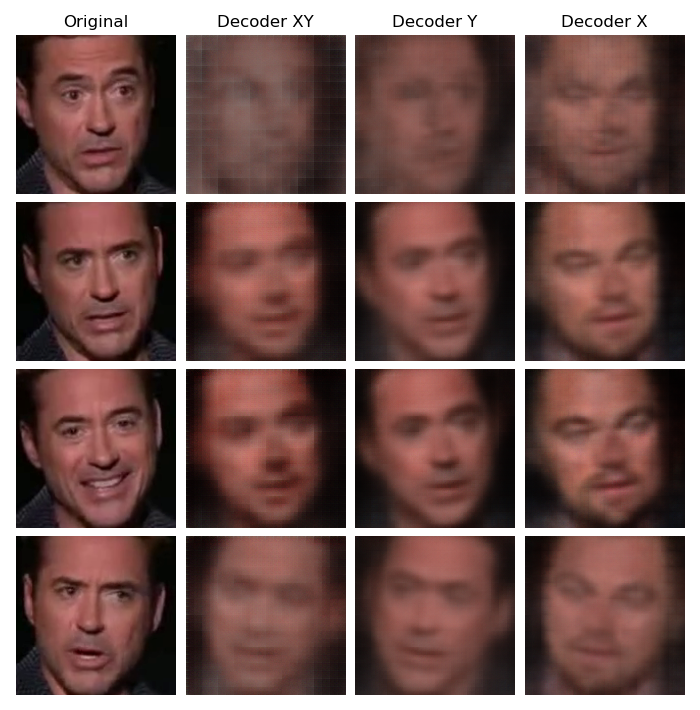
\includegraphics[width=10cm] {Results/vae_y_scene_2_600.png}
\centering
\caption{Sample 2 from subject Y after 600 epochs}
\label{fig:vae_y_scene2_600}
\end{figure}

\begin{figure}[H]
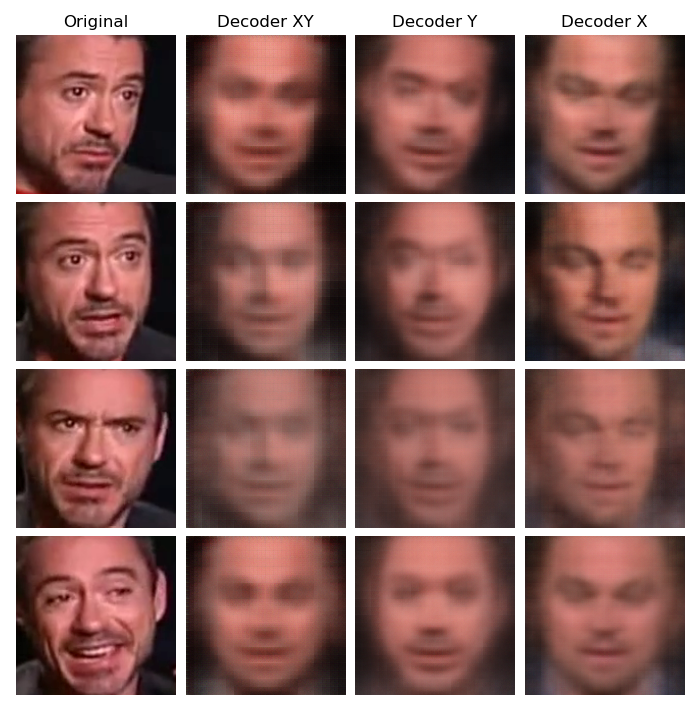
\includegraphics[width=10cm] {Results/vae_y_scene_3_600.png}
\centering
\caption{Sample 3 from subject Y after 600 epochs}
\label{fig:vae_y_scene3_600}
\end{figure}

\begin{figure}[H]
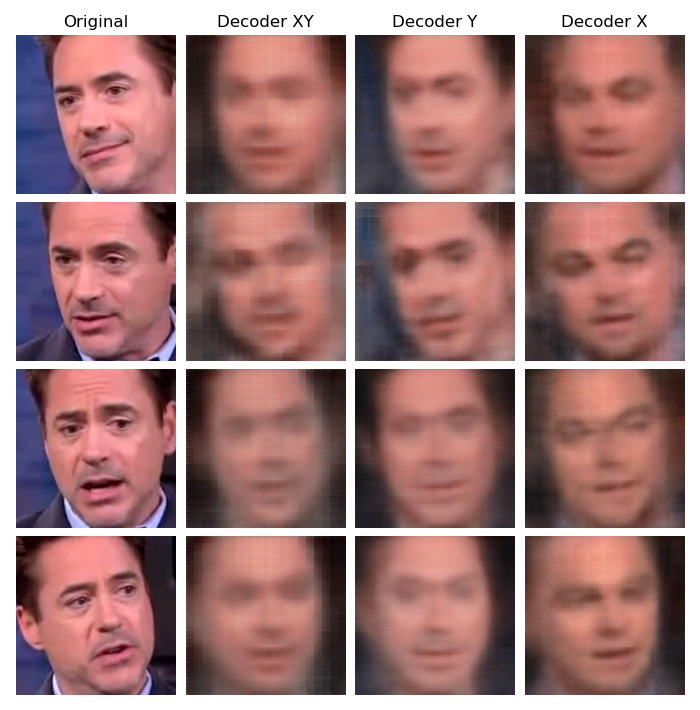
\includegraphics[width=10cm] {Results/vae_y_scene_4_600.png}
\centering
\caption{Sample 4 from subject Y after 600 epochs}
\label{fig:vae_y_scene4_600}
\end{figure}

\section{VAE-GAN}
Training process for VAE-GANs method were similar as the one described in senction \ref{Results_Autoencoder}. The encoder and decoder XY were trained were trained for 200 epochs, as shown in figure \ref{fig:vaegan_loss}. Decoder X and decoder Y were trained for 3000 epochs and during training process, trained models were saved every 100 epochs. Later, to generate final results, the most effective models were selected.

\begin{figure}[H]
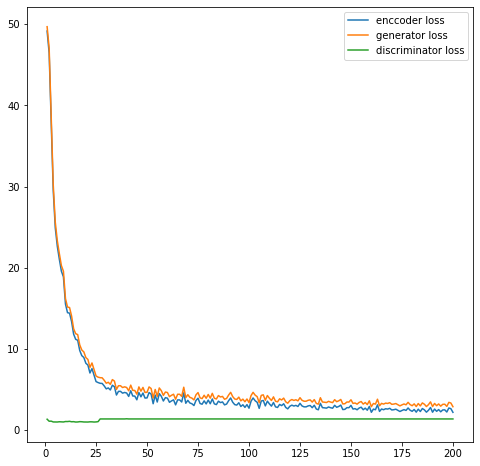
\includegraphics[width=10cm] {vaegan_loss.png}
\centering
\caption{Training process of VAE-GAN encoder and decoder XY}
\label{fig:vaegan_loss}
\end{figure}

Results presented below are in the same form as in previous section, generated over the same set of images. Deepfakes obtained from VAE-GAN method are significantly different than those from sections \ref{Results_Autoencoder} and \ref{Results_Variational_Autoencoder}. First difference is that obtained images are much less blurry and have more details characteristic for imitated person. Although the head position and overall resemblance are correctly depicted in majority of cases, face deformations of certain degree are noticeable.

\subsection{Subject X}

\begin{figure}[H]
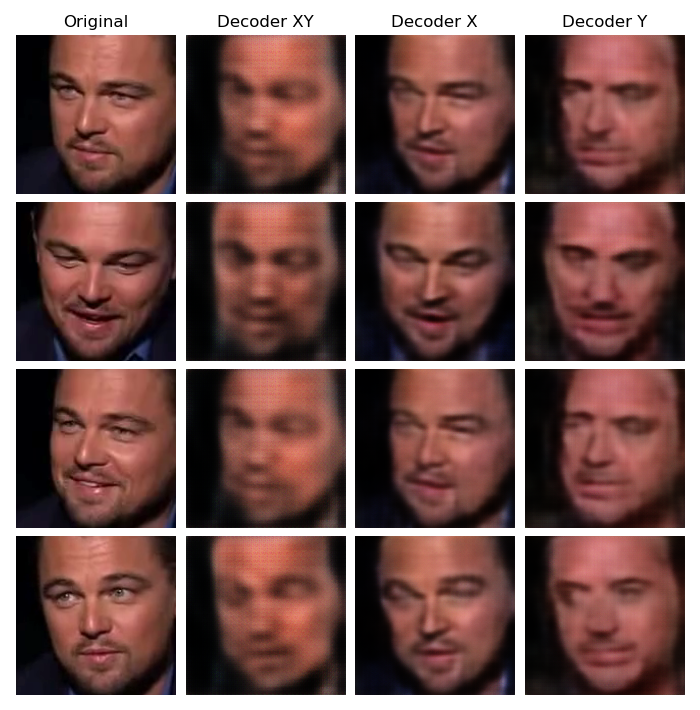
\includegraphics[width=10cm] {Results/vaegan_x_scene_1_2000.png}
\centering
\caption{Sample 1 from subject X after 2000 epochs}
\label{fig:vaegan_x_scene_1_2000}
\end{figure}

\begin{figure}[H]
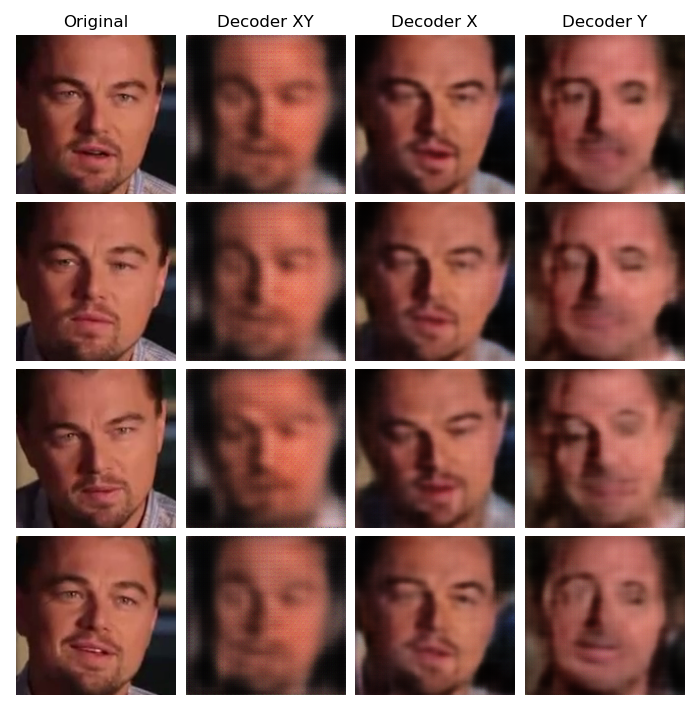
\includegraphics[width=10cm] {Results/vaegan_x_scene_2_2000.png}
\centering
\caption{Sample 2 from subject X after 2000 epochs}
\label{fig:vaegan_x_scene_2_2000}
\end{figure}

\begin{figure}[H]
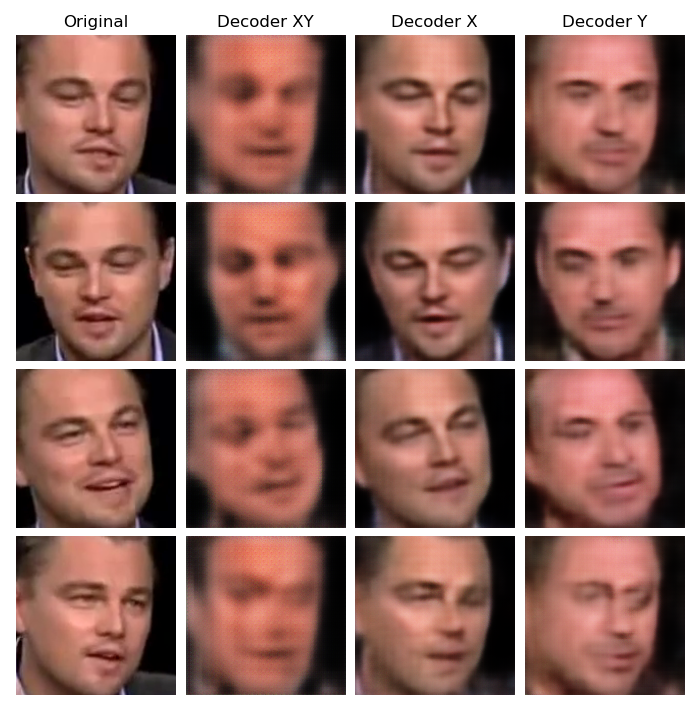
\includegraphics[width=10cm] {Results/vaegan_x_scene_3_2000.png}
\centering
\caption{Sample 3 from subject X after 2000 epochs}
\label{fig:vaegan_x_scene_3_2000}
\end{figure}

\begin{figure}[H]
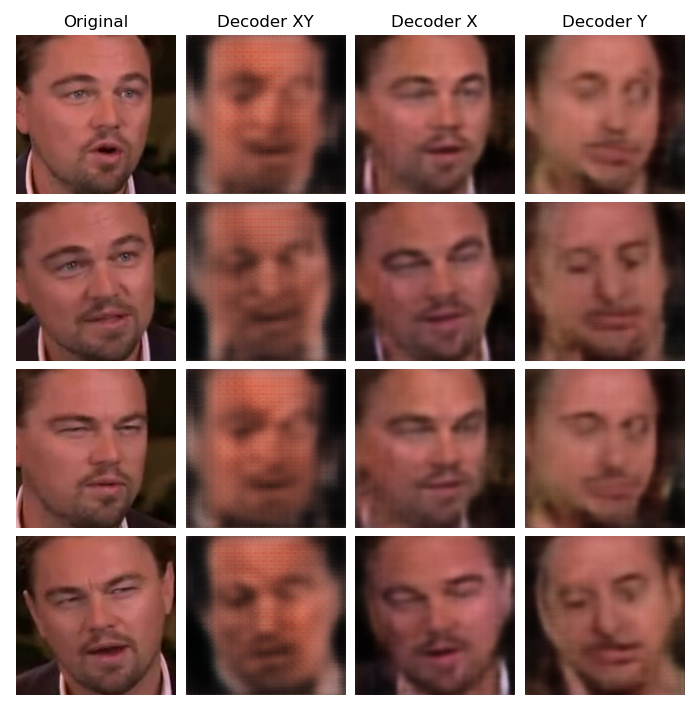
\includegraphics[width=10cm] {Results/vaegan_x_scene_4_2000.png}
\centering
\caption{Sample 4 from subject X after 2000 epochs}
\label{fig:vaegan_x_scene_4_2000}
\end{figure}

\subsection{Subject Y}

\begin{figure}[H]
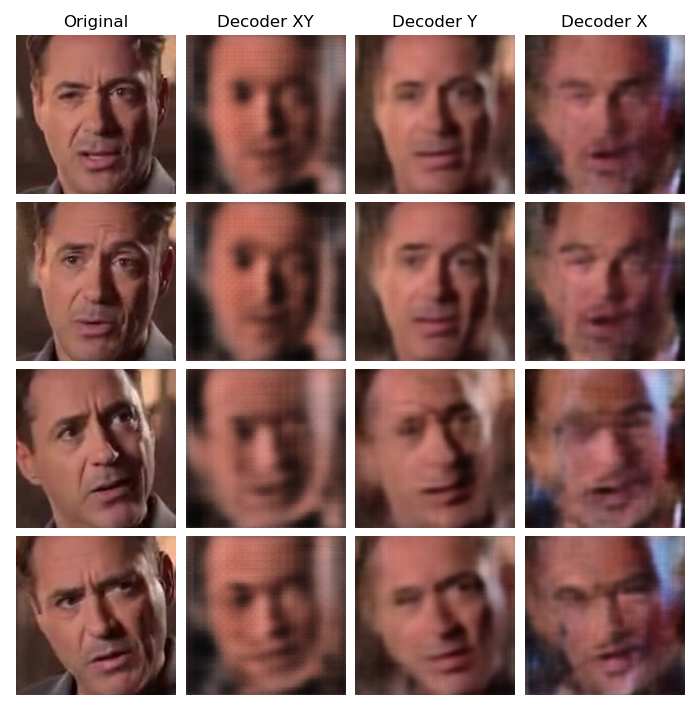
\includegraphics[width=10cm] {Results/vaegan_y_scene_1_2000.png}
\centering
\caption{Sample 1 from subject Y after 2000 epochs}
\label{fig:vaegan_y_scene_1_2000}
\end{figure}

\begin{figure}[H]
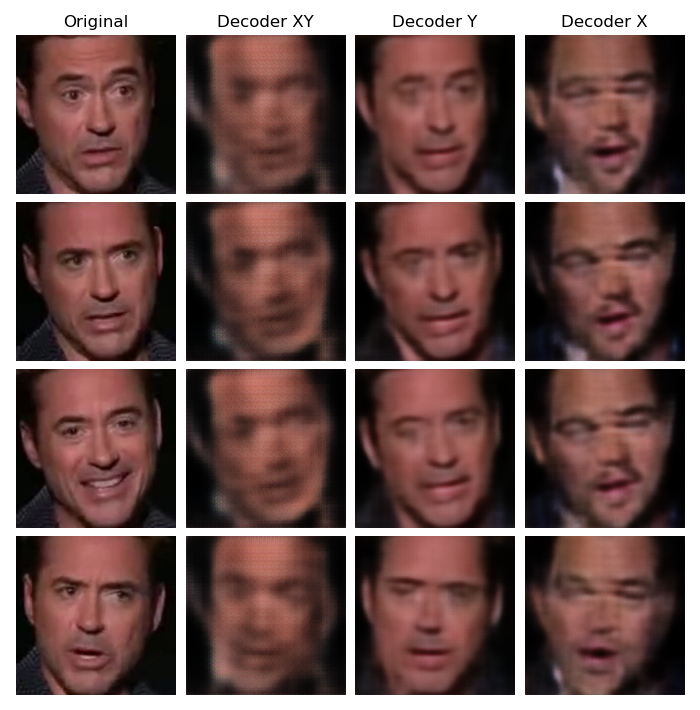
\includegraphics[width=10cm] {Results/vaegan_y_scene_2_2000.png}
\centering
\caption{Sample 2 from subject Y after 2000 epochs}
\label{fig:vaegan_y_scene_2_2000}
\end{figure}

\begin{figure}[H]
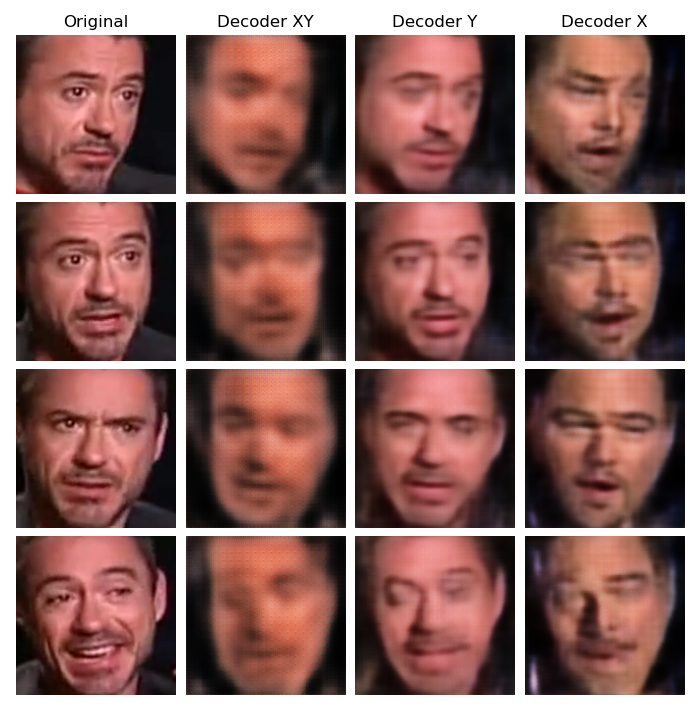
\includegraphics[width=10cm] {Results/vaegan_y_scene_3_2000.png}
\centering
\caption{Sample 3 from subject Y after 2000 epochs}
\label{fig:vaegan_y_scene_3_2000}
\end{figure}

\begin{figure}[H]
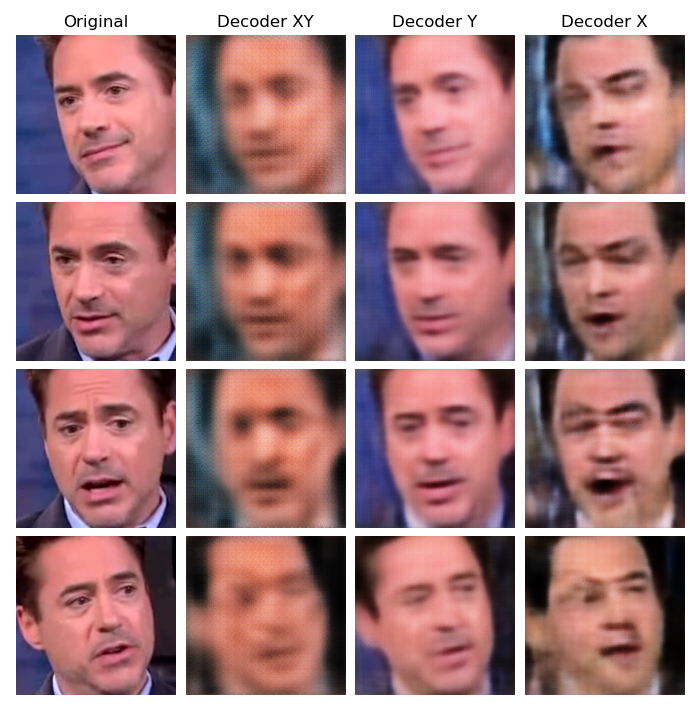
\includegraphics[width=10cm] {Results/vaegan_y_scene_4_2000.png}
\centering
\caption{Sample 4 from subject Y after 2000 epochs}
\label{fig:vaegan_y_scene_4_2000}
\end{figure}

\section{CycleGAN}
013000 powinno być ok
\subsection{Subject X}
\subsection{Subject Y}